\section{Signal Processing Methods}
\label{sec:sp}

This section provides the primary systematic contribution of this review: a taxonomy of signal processing methods applied to LCM of ball bearings, organised by processing family rather than by sensing modality. For each family the method is first described on its own terms -- its mathematical basis, assumptions, and outputs -- and then its specific applications across sensing modalities are discussed, drawing on the literature surveyed. A master cross-reference matrix linking SP method families to sensing modalities is provided in Table~\ref{tab:sp_crossref} at the end of this section.

The section contains the following categories: time-domain and frequency-domain methods (Sections~\ref{subsec:sp_time}--\ref{subsec:sp_freq}) operate directly on the measured signal; time-frequency, decomposition, and signal enhancement methods (Section~\ref{subsec:sp_tf}) address non-stationarity and improve the signal before feature extraction; physics-based and model-driven methods (Section~\ref{subsec:sp_model}) incorporate lubrication physics to convert processed signals into physically interpretable quantities; and machine learning and data fusion methods (Sections~\ref{subsec:sp_ml}--\ref{subsec:sp_fusion}) learn mappings from processed features to lubrication condition labels or regression targets. Figure~\ref{fig:sp_taxonomy} provides an overview of this taxonomy.

\begin{figure}[H]
\centering
\resizebox{\textwidth}{!}{%
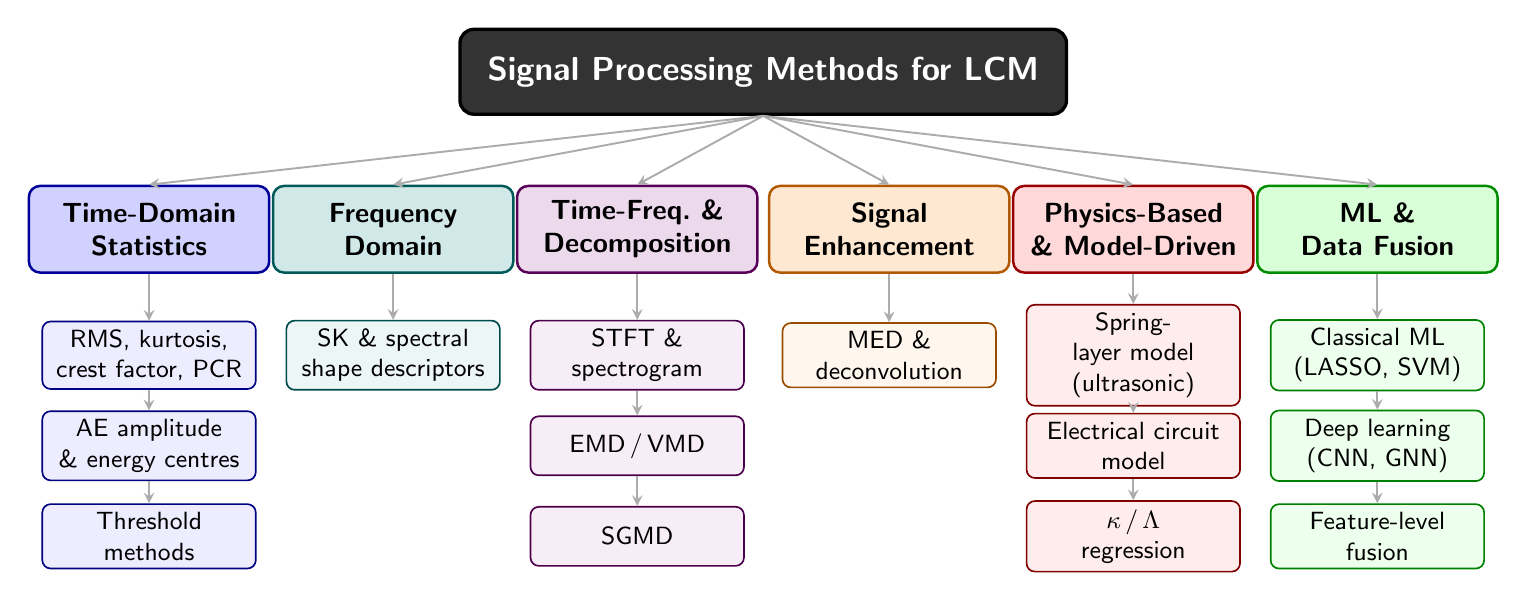
\begin{tikzpicture}[
  root/.style={rectangle, rounded corners=5pt, draw=black, line width=1.2pt,
               fill=black!80, text=white, align=center,
               font=\sffamily\bfseries\large, inner sep=10pt},
  f1/.style={rectangle, rounded corners=4pt, draw=blue!60!black, line width=0.9pt,
             fill=blue!18, align=center, font=\sffamily\bfseries\normalsize,
             text width=2.7cm, inner sep=5pt, minimum height=1.1cm},
  f2/.style={rectangle, rounded corners=4pt, draw=teal!70!black, line width=0.9pt,
             fill=teal!18, align=center, font=\sffamily\bfseries\normalsize,
             text width=2.7cm, inner sep=5pt, minimum height=1.1cm},
  f3/.style={rectangle, rounded corners=4pt, draw=violet!70!black, line width=0.9pt,
             fill=violet!15, align=center, font=\sffamily\bfseries\normalsize,
             text width=2.7cm, inner sep=5pt, minimum height=1.1cm},
  f4/.style={rectangle, rounded corners=4pt, draw=orange!70!black, line width=0.9pt,
             fill=orange!18, align=center, font=\sffamily\bfseries\normalsize,
             text width=2.7cm, inner sep=5pt, minimum height=1.1cm},
  f5/.style={rectangle, rounded corners=4pt, draw=red!60!black, line width=0.9pt,
             fill=red!15, align=center, font=\sffamily\bfseries\normalsize,
             text width=2.7cm, inner sep=5pt, minimum height=1.1cm},
  f6/.style={rectangle, rounded corners=4pt, draw=green!55!black, line width=0.9pt,
             fill=green!15, align=center, font=\sffamily\bfseries\normalsize,
             text width=2.7cm, inner sep=5pt, minimum height=1.1cm},
  m1/.style={rectangle, rounded corners=3pt, draw=blue!50!black, line width=0.6pt,
             fill=blue!7, align=center, font=\sffamily\small,
             text width=2.5cm, inner sep=3pt, minimum height=0.75cm},
  m2/.style={rectangle, rounded corners=3pt, draw=teal!60!black, line width=0.6pt,
             fill=teal!7, align=center, font=\sffamily\small,
             text width=2.5cm, inner sep=3pt, minimum height=0.75cm},
  m3/.style={rectangle, rounded corners=3pt, draw=violet!60!black, line width=0.6pt,
             fill=violet!7, align=center, font=\sffamily\small,
             text width=2.5cm, inner sep=3pt, minimum height=0.75cm},
  m4/.style={rectangle, rounded corners=3pt, draw=orange!60!black, line width=0.6pt,
             fill=orange!7, align=center, font=\sffamily\small,
             text width=2.5cm, inner sep=3pt, minimum height=0.75cm},
  m5/.style={rectangle, rounded corners=3pt, draw=red!50!black, line width=0.6pt,
             fill=red!7, align=center, font=\sffamily\small,
             text width=2.5cm, inner sep=3pt, minimum height=0.75cm},
  m6/.style={rectangle, rounded corners=3pt, draw=green!50!black, line width=0.6pt,
             fill=green!7, align=center, font=\sffamily\small,
             text width=2.5cm, inner sep=3pt, minimum height=0.75cm},
  arr/.style={->, >=stealth, line width=0.7pt, gray!65},
]

% Root
\node[root] (R) at (0,0) {Signal Processing Methods for LCM};

% Family nodes — x positions: -7.8 -4.7 -1.6 1.6 4.7 7.8
\node[f1] (F1) at (-7.8,-2.0) {Time-Domain\\Statistics};
\node[f2] (F2) at (-4.7,-2.0) {Frequency\\Domain};
\node[f3] (F3) at (-1.6,-2.0) {Time-Freq.\ \&\\Decomposition};
\node[f4] (F4) at ( 1.6,-2.0) {Signal\\Enhancement};
\node[f5] (F5) at ( 4.7,-2.0) {Physics-Based\\\& Model-Driven};
\node[f6] (F6) at ( 7.8,-2.0) {ML \&\\Data Fusion};

% Root → families
\draw[arr] (R.south) -- (F1.north);
\draw[arr] (R.south) -- (F2.north);
\draw[arr] (R.south) -- (F3.north);
\draw[arr] (R.south) -- (F4.north);
\draw[arr] (R.south) -- (F5.north);
\draw[arr] (R.south) -- (F6.north);

% Time-Domain methods
\node[m1] (M11) at (-7.8,-3.6)  {RMS, kurtosis,\\crest factor, PCR};
\node[m1] (M12) at (-7.8,-4.75) {AE amplitude\\\& energy centres};
\node[m1] (M13) at (-7.8,-5.9)  {Threshold\\methods};
\draw[arr] (F1.south)--(M11.north);
\draw[arr] (M11.south)--(M12.north);
\draw[arr] (M12.south)--(M13.north);

% Frequency-Domain methods
\node[m2] (M23) at (-4.7,-3.6)  {SK \& spectral\\shape descriptors};
\draw[arr] (F2.south)--(M23.north);

% Time-Freq & Decomposition methods
\node[m3] (M31) at (-1.6,-3.6)  {STFT \&\\spectrogram};
\node[m3] (M33) at (-1.6,-4.75) {EMD\,/\,VMD};
\node[m3] (M34) at (-1.6,-5.9)  {SGMD};
\draw[arr] (F3.south)--(M31.north);
\draw[arr] (M31.south)--(M33.north);
\draw[arr] (M33.south)--(M34.north);

% Signal Enhancement methods
\node[m4] (M41) at ( 1.6,-3.6)  {MED \&\\deconvolution};
\draw[arr] (F4.south)--(M41.north);

% Physics-Based & Model-Driven methods
\node[m5] (M51) at ( 4.7,-3.6)  {Spring-layer model\\(ultrasonic)};
\node[m5] (M52) at ( 4.7,-4.75) {Electrical circuit\\model};
\node[m5] (M53) at ( 4.7,-5.9)  {$\kappa$\,/\,$\Lambda$\\regression};
\draw[arr] (F5.south)--(M51.north);
\draw[arr] (M51.south)--(M52.north);
\draw[arr] (M52.south)--(M53.north);

% ML & Data Fusion methods
\node[m6] (M61) at ( 7.8,-3.6)  {Classical ML\\(LASSO, SVM)};
\node[m6] (M62) at ( 7.8,-4.75) {Deep learning\\(CNN, GNN)};
\node[m6] (M63) at ( 7.8,-5.9)  {Feature-level\\fusion};
\draw[arr] (F6.south)--(M61.north);
\draw[arr] (M61.south)--(M62.north);
\draw[arr] (M62.south)--(M63.north);

\end{tikzpicture}%
}
\caption{Taxonomy of signal processing method families applied to lubrication condition monitoring of rolling element bearings. Methods are organised by processing family rather than by sensing modality; the master cross-reference matrix (Table~\ref{tab:sp_crossref}) maps each family to the sensing modalities for which LCM application has been demonstrated in the reviewed literature.}
\label{fig:sp_taxonomy}
\end{figure}\todo{Update figure with final methods once paper is done.}

% ─────────────────────────────────────────────────────────────────────────────
\subsection{Time-Domain Statistical Methods}
\label{subsec:sp_time}

Time-domain statistical methods extract scalar features from a windowed segment of the raw or bandpass-filtered sensor signal. They are computationally lightweight, robust to non-stationarity within the window, and directly interpretable in physical terms. These properties make them the most practically deployed class of methods in both research and industrial LCM applications.

\subsubsection{Standard Statistical Moments and Energy Metrics}
\label{subsubsec:moments}
The most widely reported features are:
\begin{itemize}
    \item \textbf{Root mean square (RMS):} Reflects the total signal energy over the window and defined as
    \begin{equation}
    x_\mathrm{RMS} = \sqrt{\frac{1}{N}\sum_{i=1}^{N} x_i^2}.
    \end{equation}
    For passive methods, RMS increases monotonically with worsening lubrication due to increasing asperity contact energy. Widely reported for AE \cite{cornel_condition_2021,yoshioka_monitoring_2009}, vibration \cite{jakobsen_vibration_2021,jakobsen_detecting_2023,xu_vibration-based_2024}, passive ultrasound \cite{jakobsen_detecting_2023}, and thermal monitoring \cite{moussa_passive_2017}. The exception is in \cite{hou_-situ_2025} where total energy of AE signals first decreases when moving from dry to boundary lubrication but therafter increases. The decrease is due to a reduction in asperity contacts while the increase is due to higher viscous forces.
    \item \textbf{Kurtosis:} Measures the impulsiveness of the signal relative to a Gaussian distribution (for which $K=3$) and defined as
    \begin{equation}
    K = \frac{\frac{1}{N}\sum_{i=1}^{N}(x_i - \bar{x})^4}{\left(\frac{1}{N}\sum_{i=1}^{N}(x_i - \bar{x})^2\right)^2}.
    \end{equation}
    High kurtosis indicates sparse, high-amplitude transients such as those produced by asperity micro-contacts or incipient crack impacts. Usgame Sandoval et al.\ \cite{usgame_sandoval_acoustic_2013} report an $\sim$8.6-fold increase in AE kurtosis from normal to severe fault in tapered roller bearings. Yoshioka and Shimizu \cite{yoshioka_monitoring_2009} note that under grease lubrication, kurtosis of the raw vibration signal decreases as damage transitions from sparse impulsive AE to a continuous broadband noise floor -- a counter-intuitive reversal that illustrates the importance of bearing-specific calibration. Kurtosis applied to spectral representations forms the basis for higher-order spectral analysis of lubrication signals (Section~\ref{subsubsec:spectral_shape}).
    \item \textbf{Crest factor:} peak-to-RMS ratio. Sensitive to impulsive events but tends to decrease as the signal transitions from sparse impulses to continuous broadband noise, similarly to kurtosis. Applied to passive ultrasound and vibration signals for lubrication condition monitoring by Jakobsen et al.\ \cite{jakobsen_detecting_2023}.
    \item \textbf{Hjorth parameters:} three features derived from successive derivatives of the signal -- \textit{activity} (signal variance), \textit{mobility} (ratio of the standard deviation of the first derivative to that of the signal, proportional to mean frequency), and \textit{complexity} (ratio of the mobility of the first derivative to the mobility of the signal, reflecting bandwidth). Jakobsen et al.\ \cite{jakobsen_detecting_2023} apply all three to high-pass filtered passive ultrasound signals and find good correlation with $\kappa$. When combined with linear regression or a shallow neural network they predict $\kappa$ with good precision. No other paper in the reviewed literature reports Hjorth parameters for LCM.
    \item \textbf{AE amplitude and energy centres (Hou \& Zhang):} Rather than a single scalar, Hou and Zhang \cite{hou_-situ_2025} define the amplitude centre $A_c = \frac{1}{N}\sum A_i$ and energy centre $E_c = \frac{1}{N}\sum E_i$ over a 10-minute window, and form the two-dimensional pair $(A_c, E_c)$. The joint distribution in this space exhibits spatially distinct clusters for boundary, mixed, and EHL lubrication, enabling regime classification without a hard threshold. A speed-dependent weighted power-law regression of the form
    \begin{equation}
        \Lambda_E = W_A \cdot f_A(A_c, n) + W_E \cdot f_E(E_c, n),
    \end{equation}
    where $W_A, W_E$ are linear in shaft speed $n$, combines the two features to estimate the film thickness ratio $\Lambda$ with 89.3\% accuracy.
    \item \textbf{Pulse count rate (PCR):} the number of AE threshold crossings per unit time. Miettinen et al.\ \cite{miettinen_analysis_2001} show that PCR increases monotonically with grease starvation and distinguishes ten grease formulations by thickener type and base-oil viscosity. PCR is the computational minimal AE processing approach and forms the basis of the industrial threshold methods (Section~\ref{subsubsec:threshold}).
    \item \textbf{Ring-down count:} the total number of threshold crossings within a single AE burst event. Usgame Sandoval et al.\ \cite{usgame_sandoval_acoustic_2013} report a $\sim$266-fold increase in ring-down count from normal to severe fault and that ring-down count is the most sensitive single time-domain feature in their study, outperforming kurtosis and RMS.
    \item \textbf{Coefficient of quartile deviation (CQD):} a robust, distribution-shape-based measure of dispersion in the time-varying RMS, defined as $\mathrm{CQD} = (Q_3 - Q_1)/(Q_3 + Q_1)$ for quartiles $Q_1$, $Q_3$ of the RMS time series within a window. Zhang et al.\ \cite{zhang_coupled_2026} use CQD to quantify the fluctuation level of AE signals in cylindrical roller bearings and show that low-viscosity grease produces significantly higher CQD than high-viscosity grease across all analysed frequency sub-bands, consistent with a shift in the dominant AE generation mechanism.
\end{itemize}

\subsubsection{Speed and load normalisation} Time-domain features are sensitive to changes in operating speed and load independently of lubrication condition. Cornel et al.\ \cite{cornel_condition_2021} demonstrate this concretely: the relationship between AE amplitude and lubricant film thickness follows distinct curves at 500\,rpm and 3000\,rpm, making a single amplitude threshold insufficient for regime classification across speeds. This confounding effect is can be addressed by normalising features against a speed-dependent or load-dependent baseline. Hou and Zhang \cite{hou_-situ_2025} explicitly incorporate speed as a predictor in their film-thickness regression. Without such normalisation, a feature increase caused by a speed change is indistinguishable from a lubrication-related change, which limits the applicability of fixed-threshold industrial methods to constant-speed machinery.

\subsubsection{Threshold Methods}
\label{subsubsec:threshold}
The simplest operational approach is to compare a time-domain feature, commonly the ultrasound dB level or AE RMS, against a threshold established during a reference measurement under known adequate lubrication. If the feature rises a specified number of dB above the reference, relubrication is recommended \cite{lineham_ultrasonic_2008}. This is the method employed by industrial instruments such as UE Systems Ultraprobe and Sonotec's handheld devices. The advantages are simplicity, interpretability, and no requirement for labelled training data. The critical disadvantage is that the threshold carries no information about operating condition and a speed or load change might trigger a false alarm.

% ─────────────────────────────────────────────────────────────────────────────
\subsection{Frequency-Domain Methods}
\label{subsec:sp_freq}

Frequency-domain methods transform the time-domain signal into a spectral representation, enabling identification of spectral features associated with lubrication damage.

The Fourier transform and power spectral density (PSD) reveal the distribution of signal energy across frequency. In the context of LCM, two types of spectral content are of interest: (1) broadband increases in spectral energy associated with increased asperity contact under inadequate lubrication, and (2) the distribution or shape of the spectrum associated with changes in friction levels, viscous damping, asperity contacts, and lubricant contamination.

\subsubsection{Higher-Order Spectral Statistics and Spectral Shape Descriptors}
\label{subsubsec:spectral_shape}
Higher-order spectral statistics and shape descriptors characterise the spectral distribution beyond its energy content. Whether computed on a one-dimensional amplitude spectrum or per frequency bin across the time dimension of a two-dimensional STFT spectrogram, these are fundamentally shape analyses. Kurtosis measures impulsiveness and peakedness, skewness measures asymmetry, flatness the energy concentration relative to white noise, and center frequency, RMS frequency, and bandwidth-related measures the location and spread of spectral energy.

Jakobsen et al.\ \cite{jakobsen_vibration_2021} apply spectral kurtosis (SK) to vibration signals from grease-lubricated ball bearings under alternating lubrication conditions, with speed and temperature varied to span $\kappa$ from approximately 0.2 to 3.0. Band energy extracted from a lubrication-sensitive kurtogram band (7500--12000\,Hz) is correlated directly with $\kappa$ using Pearson and Spearman coefficients values. The kurtogram band energy serves as the lubrication condition indicator itself, not as a selector for downstream analysis.

Zhang et al.\ \cite{zhang_graph-data-based_2024} take a complementary approach, computing 15 spectral shape descriptors from vibration signals in the 0--3\,kHz and 10--12.8\,kHz bands and from AE signals in the 20--40\,kHz band. These include dominant frequency, band-specific energy, center frequency, RMS frequency, spectral mean and standard deviation, spectral flatness, frequency-domain skewness and kurtosis, and normalised bandwidth. The features are used in a graph-neural network for lubrication condition anomaly detection.

\subsubsection{Multi-Band Hit-Rate and Wear Particle Index}
\label{subsubsec:hitrate}
The Delft University group \cite{delft_university_of_technology_tu_delft_influence_2024} employ a three-band sensor array (40--100\,kHz, 95--180\,kHz, 180--580\,kHz) for AE monitoring of large-scale low-speed slew bearings. An AE hit is recorded when the signal in a given band exceeds a threshold with a minimum SNR of 20\,dB, and the hit rate is normalised by loading cycles to remove the effect of varying test duration. A Wear Particle Index (WPI) derived from the normalised hit rate shows linear correlation with abrasive particle mass fraction in grease. Crucially, non-abrasive (soft) particles produce negligible additional hits, demonstrating that AE hit-rate is selective for hardness contrast rather than total particle mass -- a practically important limitation for contamination monitoring.

A related but distinct use of sub-band decomposition is mechanism attribution rather than fault or wear detection. Zhang et al.\ \cite{zhang_coupled_2026} divide the 1--200\,kHz AE spectrum into 20\,kHz-wide sub-bands and, within each, fit the RMS-versus-speed trend and its coefficient of determination ($R^2$) to identify whether the asperity-load ($\sqrt{\text{speed}}$) or sliding-friction (speed$^2$) mechanism dominates. This reveals that the two AE generation mechanisms identified in Section~\ref{sec:signal_origins} are not uniformly distributed across frequency: for low-viscosity grease the lower sub-bands trend closer to the square-root relationship while higher sub-bands trend closer to quadratic, whereas for high-viscosity grease the quadratic trend holds across all sub-bands.

% ─────────────────────────────────────────────────────────────────────────────
\subsection{Time-Frequency, Decomposition, and Signal Enhancement Methods}
\label{subsec:sp_tf}

Time-frequency methods represent signal energy jointly in time and frequency, addressing the non-stationarity that characterises LCM signals arising from variable operating conditions or transient lubrication events. Decomposition methods represent the signal as components or modes and seek to identify informative parts of the signal. Signal enhancement methods deconvolute the signal to increase the signal-to-noise ratio.

\subsubsection{Short-Time Fourier Transform}
\label{subsubsec:stft}
The STFT divides the signal into short, overlapping windows and computes the FFT of each, yielding a spectrogram. The STFT is used in \cite{jakobsen_vibration_2021} as the basis for a kurtogram which conduces spectral band selection for downstream feature calculation.

\subsubsection{Signal Decomposition Methods}
\label{subsubsec:decomposition}
Empirical mode decomposition (EMD) and variants adaptively decompose a signal into intrinsic mode functions without requiring a predefined basis as with e.g. the Fourier transform. They are furthermore well suited to non-linear and non-stationary bearing signals \cite{wang_advanced_2024}. Although these methods are used in general bearing condition monitoring, no study in the reviewed LCM literature applies EMD or VMD specifically to lubrication condition estimation on a real dataset, leaving them as a potential avenue for future work. Pan et al.\ \cite{pan_symplectic_2019} provide the methodological foundation for the symplectic geometry mode decomposition (SGMD) which Yu et al.\ \cite{yu_novel_2021} apply in conjuction with empirical mode decomposition (EMD) to simualated signals from inductive debris sensors and conclude that it performs better than EMD and wavelet decompositions alone.

\subsubsection{Minimum Entropy Deconvolution}
\label{subsubsec:med}
Minimum entropy deconvolution (MED) designs a finite impulse response (FIR) filter that maximises the kurtosis of the filter output, thereby recovering the sparse impulsive excitation source from a noisy observation. In the LCM context, the impulsive sources are the transient mechanical impacts associated with asperity contacts, formation of cracks, or rolling element passage over roughened raceways under starved lubrication. Xu et al.\ \cite{xu_vibration-based_2024} demonstrate that MED applied to vibration signals significantly enhances the detection of lubrication starvation-related impulses, enabling spectral centroid and envelope features to detect starved conditions that are not detectable in the unprocessed signal. The method assumes that the source signal is sparse, which may not hold for all lubrication fault types.


% ─────────────────────────────────────────────────────────────────────────────
\subsection{Physics-Based and Model-Driven Methods}
\label{subsec:sp_model}

Physics-based methods incorporate lubricant or structural mechanics models to convert signals into physically interpretable quantities such as film thickness, lubrication regime, or lubrication adequateness. These rely on domain knowledge and are categorized into two types: physics-based measurement models which directly dictate how measurements should be interpreted, and physics-derived targets which serve as ground truths for regression or classification models.

\subsubsection{Spring Model for Ultrasonic Reflectometry}
\label{subsubsec:spring}
Active ultrasonic reflectometry estimates the reflection coefficient $R$ of an ultrasonic pulse at the raceway--lubricant interface. For a thin lubricant film, where the film thickness is much less than the acoustic wavelength, the spring model relates the estimate reflection coefficient to the film thickness and lubricant bulk modulus \cite{drinkwater_ultrasonic_2009}. Dou et al. \cite{dou_review_2022} review active ultrasonic methods for lubrication monitoring in general and note that the lubrication behaviours in ball bearings specifically are complex and almost instantaneous. Furthermore, ultrasonic reflectometry has been demonstrated to measure film thickness but has no industrial implementations. The ultrasonic spring model enables direct, calibrated film thickness estimation from the measured reflection coefficient. Validation against Hamrock--Dowson predictions is reported in \cite{dwyer-joyce_measurement_2003,zhang_ultrasonic_2015,chen_evaluation_2023}. Phase-based algorithms that improve accuracy for thin films are described in \cite{wang_accuracy-improved_2024}. Sub-Nyquist sampling to reduce data acquisition requirements while retaining film thickness accuracy is demonstrated by Chen et al.\ \cite{chen_sub-nyquist_2025}. Li et al. In general, ultrasonic reflectometry is well-covered and accurate for film thickness estimation but lacks actual industrial implementations.

\subsubsection{Electrical Circuit Models}
\label{subsubsec:electrical_model}
For electrical sensing methods (capacitance, impedance, resistance), physics-based circuit models relate a measured electrical signal to the lubricant film thickness. The bearing is modelled as a combination of electrically reactive elements whose characteristics depend on the film thickness, lubricant dielectric constant, and Hertzian contact geometry. This allows relating an eletrical probing of the bearing to lubrication film thickness. Cen et al.\ \cite{cen_ehl_2021} and Becker-Dombrowsky et al.\ \cite{becker-dombrowsky_electrical_2024} review the capacitance and impedance formulations respectively. Becker-Dombrowsky concludes that the covered methodology requires testing in other regimes than EHL, at different speeds and forces, for different types of lubricants, and for electrically induced damage of the bearings, which all constitute significant gaps before industrial applications will be possible. Maruyama et al.\ \cite{maruyama_lubrication_2023} apply the impedance model to practical deep-groove ball bearings under operating conditions. Two approaches to model calibration are reported: purely physics-based models using known material properties, and empirical calibration tests using reference lubricants to derive a relationship between the measured signal and Hamrock--Dowson-predicted film thickness \cite{cen_ehl_2021,schneider_method_2022}.

\subsubsection{Kappa and Lambda as Regression Targets}
\label{subsubsec:kappa_target}
A model-driven approach for passive sensing methods uses $\kappa$ or $\Lambda$, as the regression target for data-driven models trained on sensor features. This provides a physically grounded target variable linked to ISO standards without requiring invasive lubricant sampling. Jakobsen et al. relate spectral energy of vibration signals to $\kappa$ \cite{jakobsen_vibration_2021} and combine the Hjorth parameters with LASSO regression and shallow neural networks to predict $\kappa$ from passive ultrasound signals \cite{jakobsen_detecting_2023}. This directly bridges physics-based lubrication modelling and data-driven signal processing.

% ─────────────────────────────────────────────────────────────────────────────
\subsection{Machine Learning and Data-driven Methods}
\label{subsec:sp_ml}
Data-driven meachine learning methods learn mappings from handcrafted or raw signal features to lubrication condition labels or continuous condition estimates. They can be organised into classical machine learning and deep learning.

\subsubsection{Classical Machine Learning}
\label{subsubsec:classical_ml}
Jakobsen et al.\ \cite{jakobsen_detecting_2023} demonstrate that regularised linear regression (LASSO) on passive ultrasound features achieves good $\kappa$ prediction while providing interpretable feature weights. The feature set found through the sparsity promoting LASSO regression is furthermore used in a simple nerual network to predict $\kappa$.

\subsubsection{Deep Learning}
\label{subsubsec:dl}
Deep learning methods operate on raw signals or intermediate representations and learn features jointly with the classification or regression task. Wang et al. \cite{wang_online_2022} apply a convolutional neural network (CNN) to lubricant debris images for particle classification. Zhang et al. \cite{zhang_graph-data-based_2024} apply a graph neural network (GNN) to features from multi-sensor data (vibration, AE, temperature) lubrication degradation, leveraging sensor correlations that are not captured by independent feature extraction. Zhang et al. \cite{zhang_interpretable_2026} address the absence of labelled field lubrication faults by using a CycleGAN with multiscale residual blocks and a semantic-consistency loss to translate labelled rig signals into target-machine style, then classifying with a CNN trained solely on the generated data. This is the only reviewed method that produces usable lubrication-anomaly training data for a field deployment with no labelled field-fault examples at all. The evaluation is nonetheless not a true field test since both setups share sensor type and acquisition hardware and each lubrication state was realised on a dedicated bearing.

A consistent challenge for deep learning in LCM is the scarcity of labelled training data from real bearing degradation under controlled lubrication conditions. Controlled accelerated tests are expensive to run, and publicly available LCM datasets with varied lubrication conditions and sensing modalities are not currently available. Generative domain transfer \cite{zhang_interpretable_2026} is a response to this challenge for the specific case of lab-to-field transfer, though it remains distinct from the self-supervised and foundation-model directions discussed which target representation learning from unlabelled data rather than synthesis of labelled examples in a new domain.


% ─────────────────────────────────────────────────────────────────────────────
\subsection{Feature Fusion}
\label{subsec:feature_fusion}
Feature-level fusion concatenates feature vectors from multiple sensors into a single feature vector before the classification or regression step. Zhang et al.\ \cite{zhang_graph-data-based_2024} fuse vibration, AE, and temperature features through a graph representation. A graph attention network trained on the structure detects lubrication degradation, and the multi-sensor system outperforms any single-modality baseline. The graph-attention architecture learns which modality combinations are most informative rather than weighting all sensor contributions equally.

% ─────────────────────────────────────────────────────────────────────────────
\subsection{Master Cross-Reference Matrix}
\label{subsec:sp_crossref}

Table~\ref{tab:sp_crossref} summarises the application of SP method families to each sensing modality, as found in the reviewed literature. A filled cell indicates the combination has been demonstrated for LCM in at least one reviewed study.

\begin{table}[H]
\scriptsize
\centering
\renewcommand{\arraystretch}{1.4}
\setlength{\tabcolsep}{3pt}
\begin{tabularx}{\linewidth}{
>{\raggedright\arraybackslash}p{3cm}
 >{\centering\arraybackslash}X
 >{\centering\arraybackslash}X
 >{\centering\arraybackslash}X
 >{\centering\arraybackslash}X
 >{\centering\arraybackslash}X
 >{\centering\arraybackslash}X
 >{\centering\arraybackslash}X
 >{\centering\arraybackslash}X }
\textbf{SP Method Family}
& \rotatebox{75}{\textbf{Vibration}}
& \rotatebox{75}{\textbf{Acoustic Emission}}
& \rotatebox{75}{\textbf{Ultrasound (passive)}}
& \rotatebox{75}{\textbf{Sound / Microphone}}
& \rotatebox{75}{\textbf{Thermal}}
& \rotatebox{75}{\textbf{Active Ultrasonic}}
& \rotatebox{75}{\textbf{Electrical}}
& \rotatebox{75}{\textbf{Magnetic / Oil}}
\\
\hline
Time-domain statistics      & \checkmark & \checkmark & \checkmark &            & \checkmark &            &            &            \\
\hline
Threshold methods           &            & \checkmark & \checkmark &            &            &            &            &            \\
\hline
Spectral shape \& kurtosis  & \checkmark & \checkmark &            &            &            &            &            &            \\
\hline
Multi-band hit-rate / WPI   &            & \checkmark &            &            &            &            &            &            \\
\hline
STFT / Spectrogram          & \checkmark &            &            &            &            &            &            &            \\
\hline
Signal decomposition (SGMD) &            &            &            &            &            &            &            & \checkmark \\
\hline
MED / Deconvolution         & \checkmark &            &            &            &            &            &            &            \\
\hline
Spring-layer model          &            &            &            &            &            & \checkmark &            &            \\
\hline
Electrical circuit model    &            &            &            &            &            &            & \checkmark &            \\
\hline
$\kappa$/$\Lambda$ regression target & \checkmark & \checkmark & \checkmark &  &            &            &            &            \\
\hline
Classical ML (SVM, LASSO)   &            &            & \checkmark &            &            &            &            &            \\
\hline
Deep learning (CNN, GNN, GAN) & \checkmark & \checkmark &            &            & \checkmark &            &            & \checkmark \\
\hline
Multi-sensor fusion         & \checkmark & \checkmark &            &            & \checkmark &            &            &            \\
\hline
\end{tabularx}
\caption{Master cross-reference matrix of signal processing method families and sensing modalities for LCM of ball bearings. A \checkmark indicates the combination has been demonstrated in at least one study included in this review.}
\label{tab:sp_crossref}
\end{table}

% ─────────────────────────────────────────────────────────────────────────────
% Detailed citation-level cross-reference tables (formerly §4.4).
% Commented out as redundant with the master matrix above; retained here
% in case citation-level detail is needed for a future revision.
%
%\begin{table}[H]
%\scriptsize
%\centering
%\renewcommand{\arraystretch}{1.3}
%\setlength{\tabcolsep}{4pt}
%\begin{tabularx}{\linewidth}{|
%>{\raggedright\arraybackslash}p{2.2cm}
%| X | X | X | X | X |}
%\hline
%\textbf{SP Method}
%& \textbf{Vibration}
%& \textbf{Acoustic Emission}
%& \textbf{Temperature}
%& \textbf{Ultrasound ($>$20\,kHz)}
%& \textbf{Sound (20\,Hz--20\,kHz)}
%\\
%\hline
%\textbf{Time Domain}
%& \cite{jakobsen_detecting_2023} \cite{zhang_graph-data-based_2024} \cite{tandon_condition_2007} \cite{cornel_condition_2021} \cite{jakobsen_vibration_2021} \cite{xu_vibration-based_2024} \cite{jakobsen_low_2024} \cite{wang_advanced_2024} \cite{marticorena_rolling_2022}
%& \cite{zhang_graph-data-based_2024} \cite{miettinen_analysis_2001} \cite{tandon_condition_2007} \cite{cornel_condition_2021} \cite{kestel_condition_2025} \cite{hou_-situ_2025} \cite{delft_university_of_technology_tu_delft_influence_2024} \cite{marticorena_rolling_2022} \cite{wang_advanced_2024} \cite{yoshioka_monitoring_2009} \cite{usgame_sandoval_acoustic_2013} \cite{zhang_health_2025} \cite{renhart_monitoring_2021}
%& \cite{zhang_graph-data-based_2024} \cite{moussa_passive_2017} \cite{cen_film_2019} \cite{wang_advanced_2024}
%& \cite{jakobsen_detecting_2023} \cite{jakobsen_low_2024} \cite{lineham_ultrasonic_2008}
%&
%\\
%\hline
%\textbf{Frequency Domain}
%& \cite{zhang_graph-data-based_2024} \cite{jakobsen_vibration_2021} \cite{xu_vibration-based_2024} \cite{jakobsen_low_2024}
%& \cite{zhang_graph-data-based_2024} \cite{kestel_condition_2025} \cite{marticorena_rolling_2022} \cite{yoshioka_monitoring_2009} \cite{renhart_monitoring_2021} \cite{scheeren_acoustic_2024}
%& \cite{zhang_graph-data-based_2024}
%& \cite{jakobsen_low_2024}
%& \cite{georgiev_microphone_2017}
%\\
%\hline
%\textbf{Time-Frequency / Decomposition}
%& \cite{jakobsen_vibration_2021} \cite{xu_vibration-based_2024}
%& \cite{kestel_condition_2025} \cite{renhart_monitoring_2021}
%&
%&
%&
%\\
%\hline
%\textbf{Signal Enhancement}
%& \cite{xu_vibration-based_2024}
%& \cite{renhart_monitoring_2021}
%&
%&
%& \cite{herwig_signal_2025} \cite{pacheco-cherrez_bearing_2022}
%\\
%\hline
%\textbf{Model-Based}
%& \cite{jakobsen_detecting_2023}
%& \cite{hou_-situ_2025}
%& \cite{moussa_passive_2017}
%&
%&
%\\
%\hline
%\textbf{Machine Learning / DL}
%& \cite{zhang_graph-data-based_2024} \cite{wang_advanced_2024}
%& \cite{zhang_graph-data-based_2024} \cite{kestel_condition_2025} \cite{wang_advanced_2024} \cite{zhang_health_2025}
%& \cite{zhang_graph-data-based_2024} \cite{wang_advanced_2024}
%&
%& \cite{georgiev_microphone_2017} \cite{pacheco-cherrez_bearing_2022}
%\\
%\hline
%\textbf{Data Fusion}
%& \cite{zhang_graph-data-based_2024}
%& \cite{zhang_graph-data-based_2024}
%& \cite{zhang_graph-data-based_2024}
%&
%&
%\\
%\hline
%\end{tabularx}
%\caption{Cross-reference of signal processing methods and passive/non-invasive sensing modalities for lubrication condition monitoring in rolling element bearings.}
%\label{tab:non-invasive_methods}
%\end{table}
%
%\begin{table}[H]
%\scriptsize
%\centering
%\renewcommand{\arraystretch}{1.3}
%\setlength{\tabcolsep}{4pt}
%\begin{tabularx}{\linewidth}{|
%>{\raggedright\arraybackslash}p{2.2cm}
%| X | X | X | X | X |}
%\hline
%\textbf{SP Method}
%& \textbf{Active Ultrasonic}
%& \textbf{Electrical}
%& \textbf{Magnetic / Inductive}
%& \textbf{Optical}
%& \textbf{SAW}
%\\
%\hline
%\textbf{Time Domain}
%& \cite{shang_comprehensive_2024} \cite{lineham_ultrasonic_2008}
%& \cite{sun_online_2021}
%& \cite{sun_online_2021}
%& \cite{sun_online_2021}
%& \cite{kestel_condition_2025} \cite{lindner_a23_2011}
%\\
%\hline
%\textbf{Frequency Domain}
%&
%& \cite{sun_online_2021}
%&
%&
%&
%\\
%\hline
%\textbf{Mode Decomposition}
%&
%&
%& \cite{yu_novel_2021}
%&
%&
%\\
%\hline
%\textbf{Model-Based}
%& \cite{drinkwater_ultrasonic_2009} \cite{wang_accuracy-improved_2024} \cite{chen_evaluation_2023} \cite{dou_review_2022} \cite{zhang_ultrasonic_2015} \cite{wu_ultrasonic_2025} \cite{li_lubrication_2026}
%& \cite{cen_ehl_2021} \cite{becker-dombrowsky_electrical_2024} \cite{cen_film_2019} \cite{maruyama_lubrication_2023} \cite{maruyama_lubrication_2019} \cite{dai_situ_2024} \cite{schneider_method_2022} \cite{jablonka_quantitative_2018}
%& \cite{zhu_lubricating_2017}
%& \cite{liu_oil_2022} \cite{jablonka_quantitative_2018}
%& \cite{lindner_a23_2011} \cite{tatzgern_tribo-acoustic_2025}
%\\
%\hline
%\textbf{Sparse Sampling}
%& \cite{chen_sub-nyquist_2025}
%&
%&
%&
%&
%\\
%\hline
%\textbf{Machine Learning / DL}
%&
%&
%&
%& \cite{wang_online_2022}
%&
%\\
%\hline
%\textbf{Multi-param.\ fusion}
%&
%&
%& \cite{wang_evaluation_2018}
%&
%&
%\\
%\hline
%\end{tabularx}
%\caption{Cross-reference of signal processing methods and active or invasive sensing modalities for lubrication condition monitoring in rolling element bearings.}
%\label{tab:invasive_methods}
%\end{table}
